\chapter{Introduction and problem statement}
\label{cha:intro}
With the enormous amount of data we produce nowadays, data mining is becoming more and more prevalent.
Consequently, the goal with modern data mining methods is not only to discover information from crude data, but also to condense that information down to concise descriptions and insights.
One such method is redescription mining~\citep{ramakrishnan_turning_2004}.
In a nutshell, it aims to find different ways to describe the same things.

\chapter{Background Knowledge}
\label{cha:background}
In this chapter we are going to explore the underlying theory of the thesis.
We will go from more general knowledge to more specific concepts.
Firstly, the data mining concepts and framework are introduced.
Data mining is the process of extracting information from raw data.
Then we will dig deeper into frequent itemset mining and redescription mining, which are the two main tasks that the thesis is built upon.
\section{Data mining}
\label{sec:datamining}
Why did data mining was developed?
This chapter can give some context about that and then introduces some building blocks of the data mining framework.
\subsection{The problems}
\label{sub:the_problems}
The invention of the computer changed the way we think about storing and managing data.
Unlike books in the library or merchants in the store, data in computers can grow exponentially and instantaneously at a rate like never before.
The need for a systematic way to collect and extract useful information from a big data set started to coin in the late 1980s within companies' research departments \citep{coenen_datamining_2011}.

One of the first problems that data mining tried to solve is to create decision supports from retail clients' transactions and the sales information \citep{coenen_datamining_2011}. 
The aim is to drive the sales up, by giving out suggestions, promotions, and special pricing to the targeted customer based on their behaviors.
For example, retailers can use the system to find out which items are frequently bought together, then arrange them close to each other to create a reminding effect, which can increase the sale.
Advance a few decades later, Netflix - a streaming service company - created a system to recommend movies to users based on their favorites and activities \citep{netflix_rs_2016}.
The most difficult part of such a system is that the data is often significantly smaller than the search space.
An average person can only watch a limited number of movies, while the total number of movies is vastly bigger.
Along with that, nowadays, with the raising of low-cost communicable devices and sensors, we need to find efficient ways to deal with the data produced by them \citep{data_mining_iot_2014}.
Hence, more sophisticated and clever methods are needed; and many have been invented to deal with the growing of the complexities of the problems.

These are just a few examples of some problems that emerged in the modern time of computing and data mining.
As we can imagine, the potential of data mining is unbounded.

\subsection{The main building blocks}
\label{sub:building_blocks}

There are three main phases of data mining: \textit{data collection}, \textit{data wrangling}, and \textit{analytical processing}.

Data collection usually involves the use of hardware or software to acquire raw data.
This could be sensors' data of the environment, or user activities data from computer applications.
The choice of which data to collect is crucial and can affect greatly the quality of the result in the later phases.

After the data is collected, it is usually in a form that is difficult to be processed directly by the algorithms.
That's why we need the data preprocessing phase to make the data easier to be consumed.
This could be structuring the data into known format, e.g. multidimensional formats, time series, etc.; or removing corrupted data.

Analytical processing is the most interesting phase where useful information or insights start to emerge.
From the analytical perspective, we can categorize data mining into four "super problems": clustering, classification, \ac{apm} and outlier analysis \citep{Aggarwal15}.
Even though mining processes are different from each other, they often share some similarities and common patterns that we can generalize and apply similar techniques to them.
For example, association patterns are somewhat similar to overlapping clusters, where each pattern is corresponding to a cluster.

In the scope of this thesis, we will be more interested on the \acl{apm} problem.
\Acl{fim} \citep{borgelt_fim_2012} is the most popular model of \acl{apm}.

% Maybe introduce more type of problems here (Aggarwal15 4.1)

\section{\Acl{fim}}
\label{sec:fim}
\Acl{fim} was originally developed for marketing purposes introduced in \autoref{sub:the_problems}.
The initial goal was to analyze the market basket data to extract information about which items are frequently bought together.
Nowadays, the applications of \acl{fim} expanded to many more domains, with different variety of tasks.

\subsection{Definitions}
Formally, assume that we have a universe of all possible items $\universeOfItemset$.
For example, this can be all the possible products in a groceries store.
Suppose we have a set of $\mathit{n}$ transactions $\transaction{} = \transactionDef{}$, where $\transaction{i}$ is a composition of items from $\universeOfItemset$, with $i$ is the \ac{tid}.
This in turn, could be possible transactions at a groceries store.
Intuitively, we can see that the size of $\universeOfItemset$ is usually much larger than the size of $\transaction{}$: $|\universeOfItemset| \gg |\transaction{} |$.

Such a collection of transactions can be represented in binary representation, where all records have the same length, and each record represents a transaction.
One item in $\universeOfItemset$ will have it own same position in all records.
We can see that the length of each record is basically $|\universeOfItemset|$.
If an item appears in a transaction, it will have value $1$ in the corresponding record, otherwise $0$.
We can see this in the example \autoref{tab:market-basket-dataset}, for the first row, only Broccoli was present in the transaction, hence in the binary representation of the transaction, the first position, which corresponding to Broccoli, is set to $1$.
This representation is analogous to a matrix where the rows are the records and represents the transactions, and the columns correspond to the items.
The presence of the $\mathit{j}$th item in the $\mathit{i}$th transaction is recorded as the value in cell $\mathit{(i, j)}^{th}$.

A set of items in $\universeOfItemset$ is an \textit{itemset}. We refer to a set of $k$ items as \kItemset.
The \textit{support} of an itemset is the frequency where it appears in as a subset of a transaction in the dataset.

\begin{definition}[Support \citep{Aggarwal15}]
    The support of an itemset $\itemset$ is defined as the fraction of the transactions in the database $\transaction{} = \transactionDef{}$ that contain $\itemset$ as a subset.
\end{definition}
\begin{sloppypar}
    The support of itemset $\itemset$ is denoted by $\support{I}$.
    For example in \autoref{tab:market-basket-dataset}, $\support{\{Broccoli, Tomato\}} = 0.4$.
\end{sloppypar}
The aim of \acl{fim} is to find the itemsets with supports above a predefined \ac{minsup}.

\begin{definition}[\Acl{fim} \citep{Aggarwal15}]
    Given a set of transactions $\transaction{} = \transactionDef{}$, where each transaction $\transaction{i}$ is a subset of items from $\universeOfItemset$, determine all itemsets $\itemset$ that occur as a subset of at least a predefined fraction $\minsup$ of the transactions in $\transaction{}$.
\end{definition}

\begin{table}[tb]
    \centering
    \begin{tabular}{|l|c|c|}
        \hline
        \textbf{\ac{tid}} & \textbf{Transaction}         & \textbf{Binary representation} \\ \hline
        1            & \{Broccoli\}                 & \texttt{100}                   \\ \hline
        2            & \{Carrot\}                   & \texttt{010}                   \\ \hline
        3            & \{Tomato\}                   & \texttt{001}                   \\ \hline
        4            & \{Broccoli, Tomato\}         & \texttt{101}                   \\ \hline
        5            & \{Broccoli, Tomato, Carrot\} & \texttt{111}                   \\ \hline
    \end{tabular}
    \caption{An example of market basket dataset in binary representation}
    \label{tab:market-basket-dataset}
\end{table}
\subsection{\Acl{arm}}
\label{sub:association_rule_mining}
\Ac{fim} is the first phase of \ac{arm}.
In the following phase, the output of \ac{fim} can be further processed to find the association rules with \acl{arm}.
The result of this step is a set of rules that can be used to predict the behavior of the users.
For example, we can come to a finding that people who buy beer might also buy diapers.
Such strange finding is not quite trivial to thought of, but with the help of \acl{arm}, we can obtain it.

In order to determine whether a rule is trustworthy or not, we need to introduce a new measure: confidence.
The confidence of a rule $X \Rightarrow Y$ is the fraction of transactions containing $X$, which also contain $Y$.
\begin{definition}[Confidence \citep{Aggarwal15}]
    Let $X$ and $Y$ be two set of items.
    The confidence $conf(X \cup Y)$ of the rule $X \cup Y$ is the conditional probability of $X \cup Y$ occurring in a transaction, given that the transaction contains $X$.
    Therefore, the confidence $conf(X \cup Y)$ is defined as follows:
    \begin{equation}
        conf(X \Rightarrow Y) = \frac{sup(X \cup Y)}{sup(X)}
    \end{equation}
\end{definition}
In other words, the confidence of a rule $X \Rightarrow Y$ is the conditional probability that a transaction contains the itemset $Y$, given that it contains the itemset $X$.

For example in \autoref{tab:market-basket-dataset}, the support of \{Brocoli, Tomato\} is $2/5=0.4$, and the support of \{Broccoli, Tomato, Carrot\} is $1/5=0.2$.
Hence, the confidence of the rule $\text{\{Brocoli, Tomato\}} \Rightarrow \text{\{Carrot\}}$ is $0.2 / 0.4 = 0.5$.

Now since we have the confidence, the definition of an association rule can be presented as follows:
\begin{definition}[Association rules \citep{Aggarwal15}]
    Let $A$ and $B$ be two sets of items.
    The rule $A \Rightarrow B$ is said to be valid at support level $s$ and confidence level $c$, if the following conditions are satisfied:
    \begin{enumerate}
        \item The support of the item set $A$ is at least $s$;
        \item The confidence of $A \Rightarrow B$ is at least $c$;
    \end{enumerate}
    The first criterion ensures that a sufficient number of transactions are relevant to the rule; therefore, it has the required critical mass for it to be considered relevant to the application at hand.
    The second criterion ensures that the rule has sufficient strength in terms of conditional probabilities.
    Thus, the two measures quantify different aspects of the association rule.
\end{definition}
As we can see the confidence together with the minimum support are the core parameters of \acl{arm}.
The minimum support is used in the first phase of \acl{arm} to determine the frequent itemsets.
And the minimum confidence is used in the second phase to determine the association rules.

The frequent itemset mining phase usually takes up most of the computation time of the whole process.
Therefore, most of the research work is focused on it.
\subsection{The search space}
\label{sub:search_space}
\begin{figure}
    \centering
    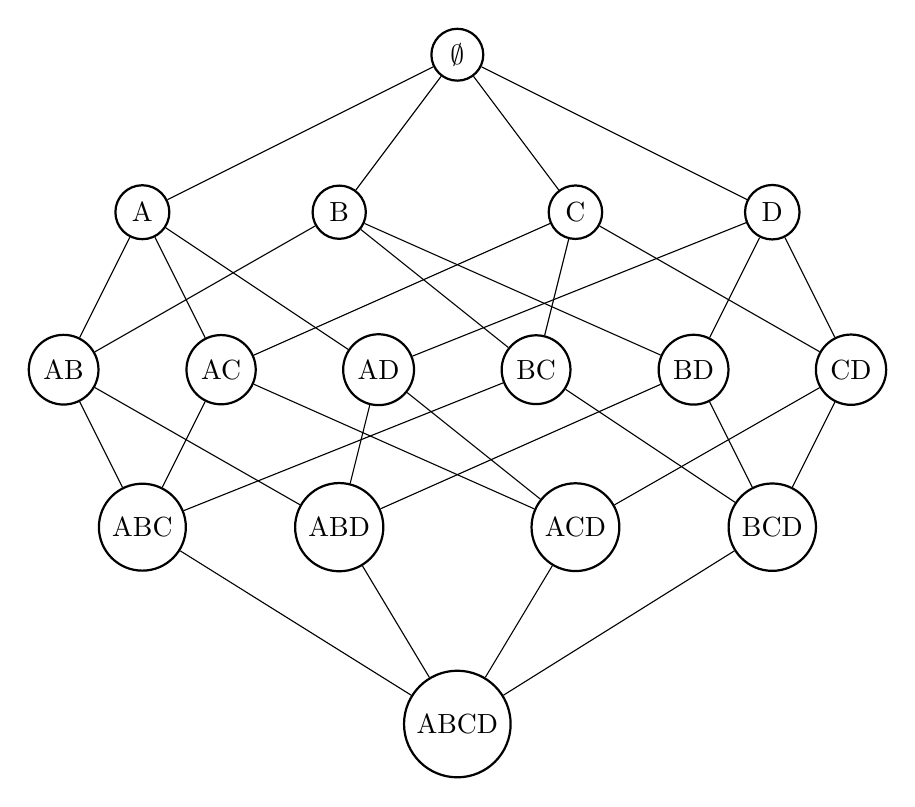
\begin{tikzpicture}[y=-1cm]
        \begin{scope}[every node/.style={circle,thick,draw}]
            \node (E) at (5,0) {$\emptyset$};
            \node (A) at (1,2) {A};
            \node (B) at (3.5,2) {B};
            \node (C) at (6.5,2) {C};
            \node (D) at (9,2) {D};
            \node (AB) at (0,4) {AB};
            \node (AC) at (2,4) {AC};
            \node (AD) at (4,4) {AD};
            \node (BC) at (6,4) {BC};
            \node (BD) at (8,4) {BD};
            \node (CD) at (10,4) {CD};
            \node (ABC) at (1,6) {ABC};
            \node (ABD) at (3.5,6) {ABD};
            \node (ACD) at (6.5,6) {ACD};
            \node (BCD) at (9,6) {BCD};
            \node (ABCD) at (5,8.5) {ABCD};
        \end{scope}
        \draw (E) -- (A);
        \draw (E) -- (B);
        \draw (E) -- (C);
        \draw (E) -- (D);
        \draw (A) -- (AB);
        \draw (A) -- (AC);
        \draw (A) -- (AD);
        \draw (B) -- (AB);
        \draw (B) -- (BC);
        \draw (B) -- (BD);
        \draw (C) -- (AC);
        \draw (C) -- (BC);
        \draw (C) -- (CD);
        \draw (D) -- (AD);
        \draw (D) -- (BD);
        \draw (D) -- (CD);
        \draw (AB) -- (ABC);
        \draw (AB) -- (ABD);
        \draw (AC) -- (ABC);
        \draw (AC) -- (ACD);
        \draw (AD) -- (ABD);
        \draw (AD) -- (ACD);
        \draw (BC) -- (BCD);
        \draw (BC) -- (ABC);
        \draw (BD) -- (ABD);
        \draw (BD) -- (BCD);
        \draw (CD) -- (ACD);
        \draw (CD) -- (BCD);
        \draw (ABC) -- (ABCD);
        \draw (ABD) -- (ABCD);
        \draw (ACD) -- (ABCD);
        \draw (BCD) -- (ABCD);
    \end{tikzpicture}
    \caption{The item lattice for a universe of 4 items.}
    \label{fig:item-lattice}
\end{figure}
% Let us use the \acl{ne} to go through it and see what will happen.
% Even though the \acl{ne} does not have any practical application, using it helps us to understand the computational complexity of \ac{fim} problem and appreciate the benefit of some optimization techniques. %, e.g. pruning or efficient support counting.

% The \acl{ne} is, unsurprisingly, very simple. It tries to check all the possible combinations to see if one is a frequent itemset or not.
% For example, with the universe of 4 items, all the possible combinations of items are represented in \autoref{fig:item-lattice}.
% In order to check the frequency of an itemset, we need to count the number of transactions that contain the itemset, this step is called \textit{support counting}.
The search space of \acl{fim} problem is enormous.
Considering a universe of items $\universeOfItemset$, there will be a total of $2^{\left\lvert \universeOfItemset \right\rvert} - 1$ possible combinations, or itemsets, excluding the empty set.
In other words, the size of the possible itemsets grows exponentially with the size of the universe.
To put this into perspective, a universe of 100 items will have a total of $2^{100} - 1$ possible itemsets, which is bigger than $10^{30}$.
At the time of writing this, the most powerful supercomputer is the Fugaku with the speed of approximately 0.4 exaflop/s \citep{monroe_fugaku_2020}.
Suppose we use this supercomputer to enumerate through the search space of all $10^{30}$ possible itemsets, and each iteration will cost us 1 flop, even though most likely it will cost more than that; this whole process will then take at least $2.5^{12}$ seconds, or at least 79 thousands years.
And all that was just for enumerating the search space, we are supposed to do the support counting at each stop and that will take much more time than the enumeration.
Realistically, the size of $\universeOfItemset$ is often much bigger than 100.
To say the least, this \acl{ne} is not practical, even for datasets over small collections of items.
There are several optimization techniques that we will discover in the following subsection.

% We will discuss some properties that can be used to optimize the frequent itemset mining phase in \autoref{sub:apriori }.
\subsection{The \acl{apriori}}
\label{sub:apriori}
As we just saw, the search space of itemsets is huge.
Hence, it is not reasonable to enumerate all possible itemsets, since a lot of candidates are inefficiently generated by the algorithm for each iteration.
Instead, we need some better strategy for traversing it.

A sensible approach to improve this is to reduce the search space by pruning some candidates, or better not generating those that we know they will not be frequent.
We know that if an itemset $I$ exists in a transaction, then all of its subsets $J_1, J_2, \dots, J_k$ must also exist in the transaction.
Hence, the number of transactions that one subset $J_i$ can be found in is always larger or equal to the corresponding value of the itemset $I$. This is called the \acl{smp}:
\begin{definition}[\Acl{smp} \citep{Aggarwal15}]
    The support of every subset $J$ of $I$ is at least equal to that of the support of itemset $I$.
    \begin{equation}
        sup(J) \geq sup(I) \quad \forall J \subseteq I
    \end{equation}
\end{definition}

The direct implication from the \acl{smp} is that every subset $J_i$ of a frequent itemset $I$ is also frequent.
This is also called the \acl{dcp} \citep{Aggarwal15}.
We can apply this property in the opposite direction, that is, if a subset $J$ is not frequent, then noen of its supersets $I_1, I_2, \dots, I_k$ can be frequent.
For example in the \autoref{fig:item-lattice}, if during the searching, we found out that $J = \{A, B\}$ is not frequent, then all the supersets of $J$, e.g. $\{A, B, C\}, \{A, B , D\}, \{A, B , C, D\}$, cannot be frequent.
We can then drop all supersets of ${J = \{A, B\}}$ from the search space.
This is a huge advantage since it allows us to stop searching early for all the supersets if we know that one of the subsets is not frequent.
What we have here is essentially the core of the \acl{apriori}, where the \acl{dcp} is applied to a \ac{ne}.
By utilizing the simple \acl{dcp} property above, the amount of candidates we have to process is drastically reduced.

% TODO add pseudo code here

The family of algorithms that enumerate the search space horizontally (breadth-first search), in turn considering candidates of size $k$, iteratively increasing the value of $k$, i.e. proceed in a level-size manner, are called the \acl{lwa}.
The \acl{apriori} is one of the earliest and most popular \acl{lwa}.
There are also approaches those traverse the search space vertically, or in other words, in a depth-first search manner.
We will later study one of such algorithm: the \acl{fpg} in \autoref{sub:fp-growth}.
% Support counting is usually a very expensive task if done naively.
% Trying to count the support more efficiently is also a good way to improve the performance.
% In \citep{brin_et_al_1997}, the \ac{dic} algorithm was presented, where itemsets are dynamically added and deleted as transactions are read instead of waiting for the scanning of the whole dataset to be completed.
% This technique proposes a concept called count-so-far which is a lower bound of the actual count of the itemset.
% If the itemset's count-so-far value is bigger than the minimum support then it will be added to the frequent itemset collection.

% One approach to prune the search space is the hash-based technique \citep{Vanitha2011USINGHB}.
% In the hash-based technique, we first scan all the transactions, we will generate all the 2-itemsets candidates for each one.
% For each 2-itemsets, we hash it into a bucket in a hash table and increase the count of the bucket by 1 if it already exists.
% The result is a table indexed by the hash value of the 2-itemsets, and the value of each bucket is the number of transactions that contain the 2-itemsets.
% We then go through the table and prune the candidates that are not frequent, i.e. the count of the bucket is less than the minimum threshold.
% This approach can reduce the number of \kItemset s substantially, especially with 2-itemsets.

% We can also use some data structure to store the candidates and/or transactions in a way that can be used to count the support efficiently.
% For instance, in \citep{bodon2003fast}, a Trie data structure was used store the candidates so that we can quickly retrieve the supports of an itemset and generate the candidates.

% There are many more other approaches to further optimize the algorithm, such as Transaction reduction \citep{zhuang_2011_transaction_reduction}, Sampling (mining on a subset of the data) \citep{zaki_1991_sampling}, etc.


\subsection{Eclat}
One big limitation of \acl*{apriori} is that it has to constantly scan the database to be able to count the supports.
The \ac{eclat} algorithm is an algorithm that does not require re-scanning the data repeatedly \citep{zaki1997}.
In \acl{apriori}, the data is in the horizontal format like in \autoref{tab:horizontal-transactional-database}, while \ac{eclat} works on vertical data format.
In the vertical transactional database, each itemset is now a key to a set of the transactions where it appears, like in \autoref{tab:vertical-transactional-database}.
The set of transactions is often called \ac{TID} set.
One important point here is that each transaction should not appear more than once, and they have to be sort alphabetically to avoid unnecessary candidate generation.
Let us see how the \ac{eclat} algorithm works by going through the example in \autoref{tab:vertical-transactional-database} step-by-step.

The first step is to transform the horizontal data into vertical data format and filter out the \ac{TID} sets smaller than the \ac{minsup}.
We can see that the support count of an itemset is simply the size of the \ac{TID} set.
Suppose the $\ac{minsup}=2$, means we will keep all the \ac{TID} sets.

Next step is the main step of the algorithm. We will intersect all the pairs of itemsets to compute the size of the \ac{TID} set for that pair.
If the size of the \ac{TID} set is smaller than the \ac{minsup}, then we will remove the itemset from the candidate set.
The result will be similar to the \autoref{tab:2-itemsets-eclat}.
We recursively repeat this step until the no more itemsets can be generated.
The output for the 3-itemsets is shown in the \autoref{tab:3-itemsets-eclat}.
From here, we can use the \ac{arm} presented in \autoref{sub:association_rule_mining} to generate meaningful rules.

Similar to the \ac{apriori} algorithm, the \ac{eclat} algorithm also works in the \ac{BFS} manner, but in each step it considers two whole vertical paths in \autoref{fig:item-lattice} at once.
The biggest drawback of \acl{eclat} is that if the TID list is too big, it can be difficult to fit it into the memory.
\begin{table}[]
    \centering
    \begin{tabular}{|l|l|}
    \hline
    TID  & Itemset        \\ \hline
    T001 & I1, I2, I5     \\ \hline
    T002 & I2, I4         \\ \hline
    T003 & I2, I3         \\ \hline
    T004 & I1, I2, I4     \\ \hline
    T005 & I1, I3         \\ \hline
    T006 & I2, I3         \\ \hline
    T007 & I1, I3         \\ \hline
    T008 & I1, I2, I3, I5 \\ \hline
    T009 & I1, I2, I3     \\ \hline
    \end{tabular}
    \caption{Transactional database in horizontal format \citep{han2012mining}}
    \label{tab:horizontal-transactional-database}
\end{table}

\begin{table}[]
    \centering
    \begin{tabular}{|l|l|}
    \hline
    Itemset & TID list                                 \\ \hline
    I1      & T100, T400, T500, T700, T800, T900       \\ \hline
    I2      & T100, T200, T300, T400, T600, T800, T900 \\ \hline
    I3      & T300, T500, T600, T700, T800, T900       \\ \hline
    I4      & T200, T400                               \\ \hline
    I5      & T100, T800                               \\ \hline
    \end{tabular}
    \caption{Transactional database in vertical format \citep{han2012mining}}
    \label{tab:vertical-transactional-database}
\end{table}

\begin{table}[]
    \centering
    \begin{tabular}{|l|l|}
    \hline
    Itemset & TID set                \\ \hline
    I1, I2  & T100, T400, T800, T900 \\ \hline
    I1, I3  & T500, T700, T800, T900 \\ \hline
    I1, I4  & T400                   \\ \hline
    I1, I5  & T100, T800             \\ \hline
    I2, I3  & T300, T600, T800, T900 \\ \hline
    I2, I4  & T200, T400             \\ \hline
    I2, I5  & T100, T800             \\ \hline
    I3, I5  & T800                   \\ \hline
    \end{tabular}
    \caption{2-itemsets step for \ac{eclat} \citep{han2012mining}}
    \label{tab:2-itemsets-eclat}
\end{table}

\begin{table}[]
    \centering
    \begin{tabular}{|l|l|}
    \hline
    Itemset     & TID set    \\ \hline
    I1, I2, I3  & T800, T900 \\ \hline
    I1, I2, I5  & T100, T800 \\ \hline
    \end{tabular}
    \caption{3-itemsets step for \ac{eclat} \citep{han2012mining}}
    \label{tab:3-itemsets-eclat}
\end{table}

\subsection{FP-Growth}
\label{sub:fp-growth}

As we can see in \autoref{sub:apriori}, the \acl{apriori} algorithm can be optimized and the search space is greatly reduced.
However, it will still have to struggle with two big problems:
\begin{itemize}
    \item The size of the candidate sets can be too large in terms of space and time to do support counting for all of them even after pruning.
    \item It still needs to scan the whole database over and over again to count the supports of each candidate.
\end{itemize}
The \acl{fpg} tackles these problems because it utilizes the divide-and-conquer approach which can reduce the size of the search space significantly.
By leveraging the \acl{fpt} data structure, the \acl{fpg} can store all the needed information in a compact way.
Furthermore, the \acl{fpt} helps us to do support counting just by traversing through the tree without scanning the whole database, this makes it become really efficient.

To understand the \acl{fpg} easily, we can go through a step-by-step example.
Suppose that we have the transactional database in \autoref{tab:horizontal-transactional-database} where T's are the transactions, and I's are the items in the transactions. 
Firstly, we formulate the frequent sets of 1-itemsets and get their support count by going through the database and count the support for each item.
We can set the minimum support to 2 to eliminate unnecessary items.

The second step is a small but important step in the \acl{fpg}, which is to sort the 1-itemsets in descending order of support count.
At this point, we will get a sorted list $C$: $C=\{\{I2:7\}, \{I1:6\}, \{I3:6\}, \{I4:2\}, \{I5:2\}\}$.
The order created in this step later will help the patterns grow in the correct order of support count.

Next, we now generate the \acl{fpt} by scanning through the transactional database and gradually construct the tree structure. Initially, we create the root of the tree with an empty node.
After that, for each transaction, we process the items in the transaction by the order of collection $C$.
For each item we process, we will check whether there is a node already for that item or not.
If not, we will create a node and link it to the parent node, the first node will be linked to the root.
If the node does exist, we will instead increase the count of that node in the tree and not creating a new branch.
Finally, we will get the \acl{fpt} structure like in \autoref{fig:fp-tree}.

\begin{figure}
    \centering
    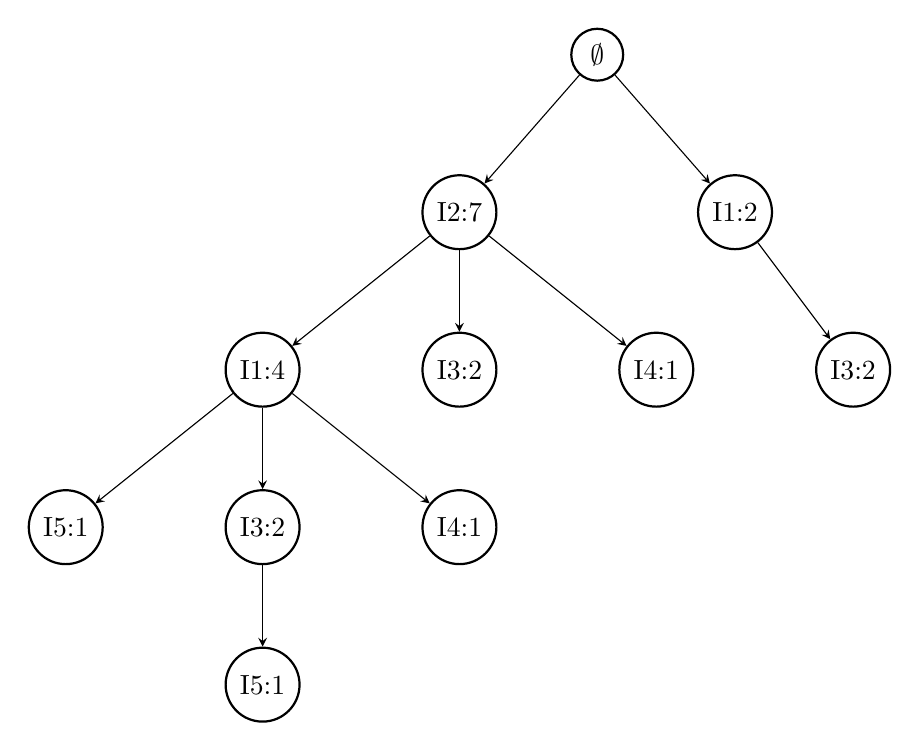
\begin{tikzpicture}[y=-1cm]
        \begin{scope}[every node/.style={circle,thick,draw}]
            \node (E) at (6.75,0) {$\emptyset$};
            \node (I2_7) at (5,2) {I2:7};
            \node (I1_2) at (8.5,2) {I1:2};
            \node (I3_2-first) at (5,4) {I3:2};
            \node (I1_4) at (2.5,4) {I1:4};
            \node (I4_1-first) at (7.5,4) {I4:1};
            \node (I3_2-second) at (10,4) {I3:2};
            \node (I5_1-first) at (0,6) {I5:1};
            \node (I3_2) at (2.5,6) {I3:2};
            \node (I4_1-second) at (5,6) {I4:1};
            \node (I5_1-second) at (2.5,8) {I5:1};
        \end{scope}
        \draw [-stealth] (E) -- (I2_7);
        \draw [-stealth] (E) -- (I1_2);
        \draw [-stealth] (I2_7) -- (I1_4);
        \draw [-stealth] (I2_7) -- (I3_2-first);
        \draw [-stealth] (I2_7) -- (I4_1-first);
        \draw [-stealth] (I1_2) -- (I3_2-second);
        \draw [-stealth] (I1_4) -- (I5_1-first);
        \draw [-stealth] (I1_4) -- (I3_2);
        \draw [-stealth] (I1_4) -- (I4_1-second);
        \draw [-stealth] (I3_2) -- (I5_1-second);
    \end{tikzpicture}
    \caption{The FP-Tree derived from scanning through the transactions.}
    \label{fig:fp-tree}
\end{figure}

Once the \acl{fpt} was created, we will move to the mining step of the algorithm.
This is the part where the divide and conquer part of the algorithm occurs.
We go through the collection $C$ in reversed order with each 1-itemset as a suffix pattern, create a \acl{cpb} of it, which is a sub-database of all the prefix patterns for the suffix pattern we are considering.
The reason we go through the collection $C$ in reversed order is because it will create good selectivity \citep{han2012mining}.
For examples, with the suffix pattern $I5$, it appears in two branches of the \acl{fpt} shown in \autoref{fig:fp-tree}: $\{I2, I1, I5: 1\}$ and $\{I2, I1, I3, I5: 1\}$.
Therefor, its \acl{cpb} will be $\{I2, I1: 1\}$ and $\{I2, I1, I3: 1\}$.
We then use the \acl{cpb} as a transactional database and formulate a \acl{cfpt} based on it.
The \acl{cfpt} is simply a single branch $\{I2:2, I1:2\}$ because $I3$ was filtered out since the support count of it is 1 which is smaller than the minimum support.
Now the task is to find all the combinations of \acl{cfpt} concatenating with the suffix then we will get the frequent patterns: $\{I2, I5: 2\}$, $\{I1, I5: 2\}$, $\{I2, I1, I5: 2\}$.
This will create a frequent pattern because both the suffix and the prefix are frequent.

We can see that we were able to find longer patterns from shorter ones, hence the name \textit{Frequent-Pattern Growth}.
By dividing the much larger database into smaller conditional databases, we were able to divide the problem recursively, which greatly reduced the complexity of the algorithm.
It has been found that the \acl{fpg} is an order of magnitude faster than the \acl{apriori} \citep{han2012mining}.

\section{Redescription mining}


\chapter{Employing ECLAT for Redescription Mining}
\label{cha:employment}

\chapter{Experiments}
\label{cha:experiments}

\chapter{Conclusions}
\label{cha:conclusions}